\documentclass{beamer}

\usepackage{braket}
\usepackage{amsmath}
\usepackage{amssymb}
\usepackage{amsthm}
\usepackage{amsfonts}
\usepackage{stmaryrd}
\usepackage{mathtools}
\usepackage{proof}
\usepackage{xfrac}
\usepackage{tensor}

\usepackage{pifont}% http://ctan.org/pkg/pifont
\newcommand{\cmark}{{\color{green} \text{\ding{51}}}}%
\newcommand{\xmark}{{\color{red} \text{\ding{55}}}}%

\usepackage{graphicx}
\usepackage{subcaption}
\graphicspath{ {./img/} }
\usepackage{tikzit}
\input{style.tikzstyles}

\usetheme{Copenhagen}
\useoutertheme{infolines}
\usecolortheme{dolphin}
\usecolortheme{rose}
%\usecolortheme{orchid}
%\usecolortheme{lily}

%\newcommand{\note}[1]{{\color{red} #1}}
\newcommand{\mono}[1]{\texttt{#1}}

%braket notation
\newcommand{\ketbra}[2]{\ket{#1}\!\!\bra{#2}}
\newcommand{\proj}[1]{\ketbra{#1}{#1}}
\newcommand{\kp}{\ket{\psi}}
\newcommand{\kf}{\ket{\phi}}
\newcommand{\kz}{\ket{0}}
\newcommand{\ko}{\ket{1}}
\newcommand{\kpl}{\ket{+}}
\newcommand{\km}{\ket{-}}
\newcommand{\oost}{\frac{1}{\sqrt{2}}}

%hilbert spaces, density matrices and sops
\newcommand{\calH}{\mathcal{H}}
\newcommand{\hilbert}{\calH}
\newcommand{\calHt}{\mathcal{H}^2}
\newcommand{\Hto}[1]{\mathcal{H}^{\otimes #1}}
\newcommand{\calDH}{\mathcal{D}(\mathcal{H})}
\newcommand{\calSH}{\mathcal{S}(\mathcal{H})}
\newcommand{\sop}{\mathcal{E}}
\newcommand{\cnot}{\text{CNOT}}

%process algebras
\newcommand{\ITE}[3]{\textbf{If }{#1}\textbf{ Then } {#2} \textbf{ Else } {#3}}
\newcommand{\bigzero}{\mbox{\normalfont\bfseries 0}}
\newcommand{\qsum}[1]{\tensor[_{#1}]{\boxplus}{}}
\newcommand{\psum}[1]{\tensor[_{#1}]{\oplus}{}}
\newcommand{\nil}{\mathbf{0}}
\newcommand{\sem}[1]{\llbracket#1\rrbracket}
\newcommand{\sema}[1]{\llparenthesis\,#1\,\rrparenthesis}
\newcommand{\rel}{\mathcal{R}}
\newcommand{\lrel}{\mathring{\rel}}
\newcommand{\conf}{\mathcal{C}}
\newcommand{\confw}[1]{\big\langle#1\big\rangle}
\newcommand{\blank}{{-}}
\newcommand{\qlift}[1]{\stackrel{\scriptscriptstyle \boxplus}{#1}}
\newcommand{\slift}[1]{\stackrel{\scriptscriptstyle \circ}{#1}}
\newcommand{\sqlift}[1]{\hat{#1}}
\newcommand{\barb}[3]{#3\downarrow_{#1, #2}}
\newcommand{\proc}[1]{\text{\textbf{#1}}}
\newcommand{\ite}[3]{\textbf{if } #1 \textbf{ then } #2 \textbf{ else } #3}

%bisimulation symbols
\newcommand{\simps}{\sim_{PS}}
\newcommand{\simqs}{\sim_{QS}}
\newcommand{\distr}{\mathfrak{D}}


%Information to be included in the title page:
\title{Exploring Quantum Process Calculi}
\author{Gabriele Tedeschi}
\institute{University of Pisa}
\date{October 7, 2022}	

\begin{document}

\frame{\titlepage}

\begin{frame}{Table Of Contents}
\tableofcontents
\end{frame}

\section{Quantum computing fundamentals}
\begin{frame}{Qubits}
The simplest quantum system is a \textbf{qubit}. Like a bit, a qubit has two separate states, $\kz$ and $\ko$.


A qubit can also be in a linear combination of states, knows as a \textbf{superposition}.
\begin{columns}
\column{0.5\textwidth}
\[ \kpl = \oost \kz + \oost \ko \]
\[\km = \oost \kz - \oost \ko \]

\column{0.5\textwidth}
\begin{figure}
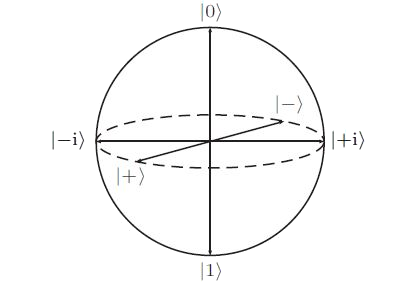
\includegraphics[scale=0.6]{bloch_no_bkg}
\end{figure} 
\end{columns}
\end{frame}



\begin{frame}{Measurements}
A qubit in superposition cannot be directly observed, because when it get \textbf{measured}, it \textbf{decays} in one of its basis states.

\bigskip

\ctikzfig{measurement_gen}

\bigskip

For example, when measuring the state $\kpl = \oost \kz + \oost \ko$, we get either $\kz$ or $\ko$ with the same probability. 
\end{frame}



\begin{frame}{No Cloning theorem}
\begin{block}{No-Cloning}
Quantum information cannot be \textbf{duplicated}. That is, given a qubit $q_1$ in state $$\kp = \alpha\kz + \beta\ko$$ it is impossible to prepare a qubit $q_2$ in the same state, without destroying the information in $q_1$.
\end{block}

\bigskip
This means that, contrary to classical bits, qubits cannot be freely copied, stored or broadcasted to multiple receivers.
\end{frame}


\section{Linear qCCS}
\begin{frame}{Linear qCCS: Type System}
\begin{block}{lqCCS}
\textbf{Linear qCCS} (lqCCS) is an asynchronous value-passing calculus, equipped with a \textbf{linear type system} to regulate quantum communication. It features parallelism, non-determinism and quantum operations.
\end{block}

\bigskip

\pause
The type system is needed to prevent \textbf{duplication} of quantum information: after receiving a qubit, a process must send it \textbf{exactly once}. 

\begin{align*}
& c?q.H(q).c!q  & &  a?q.\big(b!q \parallel c!q\big) \  & & c?q.H(q).\nil \  \\
& \qquad\onslide<3->{\cmark}  & & \qquad\onslide<4->{\xmark} & & \qquad\onslide<5->{\xmark}
\end{align*}

\end{frame}

\begin{frame}{Linear qCCS: Linearity}
In previous calculi, there were \textbf{ambiguous} processes like 
\[
 P = c?q.X(q).\nil \qquad Q = c?q.H(q).\nil
\]
\pause
Are $P$ and $Q$ \textbf{observationally equivalent}? It depends on what happens to $q$, different calculi followed different assumptions.

\bigskip

\pause
In lqCCS, the programmer must \textbf{explicitly} describe what happens to each qubit
\[
 P' = c?q.X(q).c!q \qquad Q' = c?q.H(q).c!q
\]
\[
 P'' = c?q.X(q).disc(q) \qquad Q'' = c?q.H(q).disc(q)
\]
\end{frame}

\begin{frame}{Linear qCCS: Probabilistic Transition System}
\begin{columns}
\column{0.4\textwidth}
\begin{itemize}
\item<1-> Transition system made of \textbf{configurations}, of the form $\confw{\kp, P}$
\item<2-> \textbf{Reduction system}, without labels
\item<3-> Probabilistic behaviour, a configuration can evolve in a \textbf{distribution} of configurations
\end{itemize}

\column{0.6\textwidth}
\only<4->{
  \ctikzfig{transition_system}}
\end{columns}
\end{frame}


\begin{frame}{Linear qCCS: Bisimilarity via barbs and contexts}

\begin{block}{Saturated Bisimilarity}
Two processes are \textbf{saturated bisimilar} if they express the same \textbf{observable behaviour} under any \textbf{context} 
\pause
\begin{itemize}
\item 
Observable behaviour (barb): the capability of sending some value on a specific channel
\pause
\item Context: a "program" with a hole, like $[\blank] \parallel R$. We compare $P$ and $Q$ "inside" this context, i.e. we study $P \parallel R$ and $Q \parallel R$.
\end{itemize}
\end{block}


\pause
The two processes seen before \[
 P' = c?q.X(q).c!q \qquad Q' = c?q.H(q).c!q
\]
are not bisimilar, because there is a context $R$ which tells them apart
\[ R = c?q.M_{01}[q \rhd x].\left( disc(q)\parallel \ite{x = 0}{a!0}{b!0}\right)\]

\end{frame}


\section{The problem with probabilistic bisimilarity}
\begin{frame}{Probabilistic Bisimilarity}
Thanks to lqCCS, we can compare the existing bisimilarities, and find the more appropriate for the quantum setting. 
\pause

Consider the two configurations 
\begin{align*}
\conf = \confw{\kpl, M_{01}[q \rhd x].c!q} &\rightarrow \confw{\kz, c!q} \psum{\frac{1}{2}} \confw{\ko, c!q} \\
\conf' = \confw{\kz, M_{\pm}[q \rhd x].c!q} &\rightarrow \confw{\kpl, c!q} \psum{\frac{1}{2}} \confw{\km, c!q}
\end{align*}
\pause
According to the usual notion of \textbf{probabilistic bisimilarity}, two distributions are bisimilar if they assign the same probability to bisimilar processes. In our example, the two configurations  are \textbf{not} bisimilar, because they evolve in two non-bisimilar distributions.

\end{frame}

\begin{frame}{Indistinguishable distributions}

According to quantum mechanics, it's impossible to distinguish the two sources $S$ and $S'$:
\begin{align*}
S &\text{ emits a qubit $\kz$ or $\ko$ with the same probability}\\
S' &\text{ emits a qubit $\kpl$ or $\km$ with the same probability}
\end{align*}
Suppose we receive a qubit from either $S$ or $S'$, and measure it in the $01$ basis. If we measure a qubit from $S$, it would result in either $\kz$ or $\ko$. If we measure a qubit from $S'$, a $\kpl$ qubit would decay in either $\kz$ or $\ko$, and a $\km$ qubit would decay in either $\kz$ or $\ko$ as well.

\pause
\begin{block}{Inadequacy of Probabilistic Bisimilarity}
The usual notion of probabilistic bisimilarity is too fine, when comparing distributions of quantum configurations.
\end{block}
\end{frame}

\section{Solution I: Quantum Bisimilarity}


\begin{frame}{Solution I: Quantum Bisimilarity}
\begin{block}{Quantum Bisimilarity}
We introduce an \textit{equivalence} relation $$\equiv \, \subseteq \distr(Conf) \times \distr(Conf)$$ and a new notion of \textbf{quantum bisimilarity}. Two processes are quantum bisimilar if they evolve in distributions that are bisimilar \textbf{up to equivalence}.
\end{block}
\pause
\begin{small}
\begin{align*}
\confw{\kpl, M_{01}[q \rhd x].c!q} \rightarrow \confw{\kz, c!q} \psum{\frac{1}{2}} \confw{\ko, c!q} \only<3->{\equiv \confw{\kpl, c!q} &\psum{\frac{1}{2}} \confw{\km, c!q}}
\\
\only<2>{\not\sim \hspace*{1.7cm}}\only<4>{&\sim}
\\
\confw{\kz, M_{\pm}[q \rhd x].c!q} \rightarrow \confw{\kpl, c!q} \psum{\frac{1}{2}} \confw{\km, c!q} \only<3->{\equiv \confw{\kpl, c!q} &\psum{\frac{1}{2}} \confw{\km, c!q}}
\end{align*}
\end{small}

\end{frame}

\section{Solution II: mQPA}
\pause
\begin{frame}{Minimal Quantum Process Algebra}
\begin{block}{Solution II: mQPA}
We introduce a new calculus, equipped with a minimal set of features: communication, non-determinism and quantum measurement.

In mQPA, the transitions are of the form
\[\rightarrow \subseteq S \times \distr(S)^\mathcal{H}\]
i.e. the probabilistic observable behaviour is \textbf{parametric} with respect to an input quantum state.		
\end{block}
\pause
In mQPA, the previous example can be rewritten as
\begin{align*}
	  (S \qsum{\proj{0}} S')(\kpl) = S \psum{\frac{1}{2}} S'\\
	  (S \qsum{\proj{+}} S')(\kz) = S \psum{\frac{1}{2}} S'\\
\end{align*}
\end{frame}


\section{Conclusions}
\begin{frame}{What have we seen}
\begin{itemize}
\item<2-> \textbf{lqCCS}, an asynchronous linear calculus inspired by  qCCS. It rephrases the syntax e semantics of previous calculi in a more standard formalism, and allows to compare different notions of bisimilarity. 
\item<3-> Even though quantum systems exhibit a probabilistic behaviour, \textbf{probabilistic bisimilarity} is not really well suited for the quantum setting. 
\item<4-> \textbf{quantum bisimilarity} relaxes the conditions of probabilistic bisimilarity, better representing quantum systems.
\item<4-> \textbf{mQPA}, a minimal calculus, pursuing a foundational approach on which are the dynamics and observable properties of quantum systems.
\end{itemize}
\end{frame}


\begin{frame}{Future work}
\begin{itemize}
\item<2-> We will work on \textbf{non-strong extensions} (weak or barbed bisimilarity), as for example protocol implementation should be weakly bisimilar to its specification.
\item<3->  From weak transitions, it is possible to define reachability, temporal logics and \textbf{model checking}.
\item<4->  Saturated bisimilarity can be cumbersome to prove, it will be interesting to explore how the existing \textbf{proof techniques} adapt to the quantum setting.
\item<5->  We will investigate the relation between \textbf{mQPA} semantics and the usual, configuration-based semantics, together with their respective bisimilarities.
\end{itemize}
\end{frame}

\begin{frame}
\bigskip
\begin{Large}
\begin{center}
Thank you for your attention!
\end{center}
\end{Large}
\end{frame}


\end{document}
